\section{Date: 2026-09-13}
\noindent \textbf{Series ID: CIS2010000500000I} 

\noindent This series is titled Employment Cost Index: Total compensation for Private industry workers in Production, transportation, and material moving and has a frequency of Quarterly. The units are Index Dec 2005=100 and the seasonal adjustment is Seasonally Adjusted.The observation start date is 2002-01-01 and the observation end date is 2026-04-01.The popularity of this series is 1. \\ 

\noindent \textbf{Series ID: ECIGVTCOM} 

\noindent This series is titled Employment Cost Index: Compensation: State and Local Government: All Workers and has a frequency of Quarterly. The units are Index Dec 2005=100 and the seasonal adjustment is Seasonally Adjusted.The observation start date is 2001-01-01 and the observation end date is 2026-04-01.The popularity of this series is 5. \\ 

\subsection{Raw Regression}
\noindent Regresses the two series against each other directly. A significant result here can come just as easily from both series sharing a long-run trend as from any real relationship.

\begin{center}
\begin{tabular}{lclc}
\toprule
\textbf{Dep. Variable:}                 & value\_fred\_ECIGVTCOM & \textbf{  R-squared:         } &     0.989   \\
\textbf{Model:}                         &          OLS           & \textbf{  Adj. R-squared:    } &     0.989   \\
\textbf{Method:}                        &     Least Squares      & \textbf{  F-statistic:       } &     8834.   \\
\textbf{Date:}                          &    Sun, 13 Sep 2026    & \textbf{  Prob (F-statistic):} &  2.63e-96   \\
\textbf{Time:}                          &        15:09:51        & \textbf{  Log-Likelihood:    } &   -230.11   \\
\textbf{No. Observations:}              &             98         & \textbf{  AIC:               } &     464.2   \\
\textbf{Df Residuals:}                  &             96         & \textbf{  BIC:               } &     469.4   \\
\textbf{Df Model:}                      &              1         & \textbf{                     } &             \\
\textbf{Covariance Type:}               &       nonrobust        & \textbf{                     } &             \\
\bottomrule
\end{tabular}
\begin{tabular}{lcccccc}
                                        & \textbf{coef} & \textbf{std err} & \textbf{t} & \textbf{P$> |$t$|$} & \textbf{[0.025} & \textbf{0.975]}  \\
\midrule
\textbf{const}                          &       7.0722  &        1.299     &     5.444  &         0.000        &        4.494    &        9.651     \\
\textbf{value\_fred\_CIS2010000500000I} &       0.9540  &        0.010     &    93.989  &         0.000        &        0.934    &        0.974     \\
\bottomrule
\end{tabular}
\begin{tabular}{lclc}
\textbf{Omnibus:}       & 47.674 & \textbf{  Durbin-Watson:     } &    0.025  \\
\textbf{Prob(Omnibus):} &  0.000 & \textbf{  Jarque-Bera (JB):  } &   11.046  \\
\textbf{Skew:}          & -0.530 & \textbf{  Prob(JB):          } &  0.00399  \\
\textbf{Kurtosis:}      &  1.742 & \textbf{  Cond. No.          } &     643.  \\
\bottomrule
\end{tabular}
%\caption{OLS Regression Results}
\end{center}

Notes: \newline
 [1] Standard Errors assume that the covariance matrix of the errors is correctly specified.

\begin{figure}
\centering
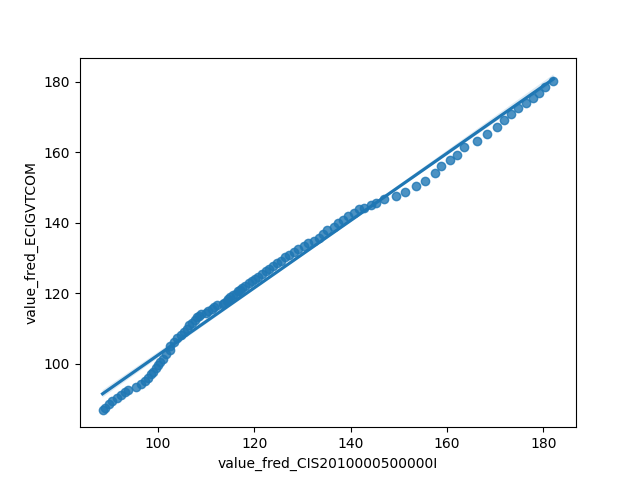
\includegraphics[scale = 0.9]{plots/plot_2026-09-13.png}
\caption{Raw Regression Plot for 2026-09-13}
\end{figure}
\newpage
\subsection{Detrended Regression}
\noindent Regresses the residuals of each series after removing its own linear time trend, so a shared trend can no longer drive the result on its own. A relationship that stays significant here is better evidence of a genuine link between the two series.

\begin{center}
\begin{tabular}{lclc}
\toprule
\textbf{Dep. Variable:}                            & value\_fred\_ECIGVTCOM\_detrended & \textbf{  R-squared:         } &     0.834   \\
\textbf{Model:}                                    &                OLS                & \textbf{  Adj. R-squared:    } &     0.832   \\
\textbf{Method:}                                   &           Least Squares           & \textbf{  F-statistic:       } &     481.9   \\
\textbf{Date:}                                     &          Sun, 13 Sep 2026         & \textbf{  Prob (F-statistic):} &  3.38e-39   \\
\textbf{Time:}                                     &              15:09:51             & \textbf{  Log-Likelihood:    } &   -190.53   \\
\textbf{No. Observations:}                         &                   98              & \textbf{  AIC:               } &     385.1   \\
\textbf{Df Residuals:}                             &                   96              & \textbf{  BIC:               } &     390.2   \\
\textbf{Df Model:}                                 &                    1              & \textbf{                     } &             \\
\textbf{Covariance Type:}                          &             nonrobust             & \textbf{                     } &             \\
\bottomrule
\end{tabular}
\begin{tabular}{lcccccc}
                                                   & \textbf{coef} & \textbf{std err} & \textbf{t} & \textbf{P$> |$t$|$} & \textbf{[0.025} & \textbf{0.975]}  \\
\midrule
\textbf{const}                                     &    4.162e-13  &        0.173     &  2.41e-12  &         1.000        &       -0.343    &        0.343     \\
\textbf{value\_fred\_CIS2010000500000I\_detrended} &       0.6428  &        0.029     &    21.952  &         0.000        &        0.585    &        0.701     \\
\bottomrule
\end{tabular}
\begin{tabular}{lclc}
\textbf{Omnibus:}       &  4.629 & \textbf{  Durbin-Watson:     } &    0.041  \\
\textbf{Prob(Omnibus):} &  0.099 & \textbf{  Jarque-Bera (JB):  } &    2.345  \\
\textbf{Skew:}          &  0.034 & \textbf{  Prob(JB):          } &    0.310  \\
\textbf{Kurtosis:}      &  2.245 & \textbf{  Cond. No.          } &     5.89  \\
\bottomrule
\end{tabular}
%\caption{OLS Regression Results}
\end{center}

Notes: \newline
 [1] Standard Errors assume that the covariance matrix of the errors is correctly specified.

\begin{figure}
\centering
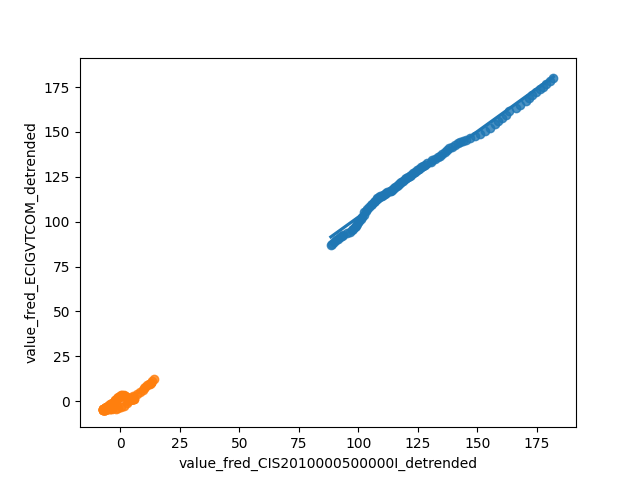
\includegraphics[scale = 0.9]{plots/plot_2026-09-13_detrended.png}
\caption{Detrended Regression Plot for 2026-09-13}
\end{figure}
\newpage
